
\documentclass[tikz, border=1mm]{standalone}

\usepackage{amsmath}

\usepackage{tikz}

\usetikzlibrary{calc,angles,quotes,shapes.geometric}

\usepackage{tkz-euclide}

\begin{document}

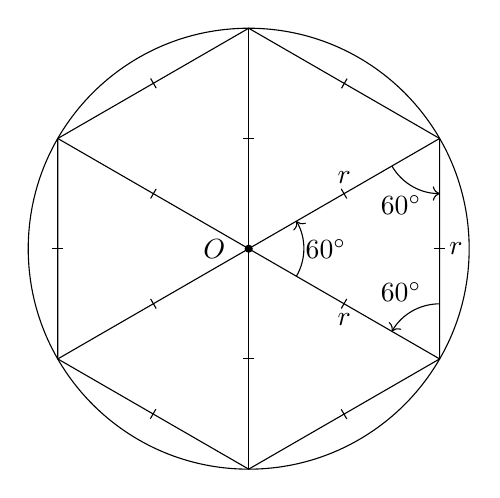
\begin{tikzpicture}[scale=1.4]

	% parameters
	\def\numsides{6}
	\def\radius{2}
	\def\rotation{90}

	% coordinates
	\coordinate (O) at (0,0);
	\foreach \i in {1,...,\numsides} {
		\coordinate (P\i) at ({360/\numsides*(\i-1)+\rotation}:\radius);
	}

	% circle
	\draw (O) circle (\radius);

	% polygon
	\draw (P1) \foreach \i in {2,...,\numsides} { -- (P\i) } -- cycle;

	% radiuses
	\foreach \i in {1,...,\numsides} { \draw (O) -- (P\i); }

	% vertices labels
	\node[label={[label distance=0.5mm]left:$O$}] at (O) {};
	\filldraw (O) circle (0.9pt);

	\node[above] at ($(O)!0.5!(P6)$) {$r$};
	\node[below] at ($(O)!0.5!(P5)$) {$r$};
	\node[right] at ($(P5)!0.5!(P6)$) {$r$};

	% segments marks
	\foreach \i in {1,...,\numsides} {
		\tkzMarkSegments[mark=|, size=2pt](O,P\i)
	}

	\tkzMarkSegments[mark=|, size=2pt](P1,P2)
	\tkzMarkSegments[mark=|, size=2pt](P2,P3)
	\tkzMarkSegments[mark=|, size=2pt](P3,P4)
	\tkzMarkSegments[mark=|, size=2pt](P4,P5)
	\tkzMarkSegments[mark=|, size=2pt](P5,P6)
	\tkzMarkSegments[mark=|, size=2pt](P6,P1)

	\pic[draw, ->, "$60^\circ$", angle radius=0.7cm, angle eccentricity=1.4]
	{angle = P5--O--P6};

	\pic[draw, ->, "$60^\circ$", angle radius=0.7cm, angle eccentricity=1.4]
	{angle = P6--P5--O};

	\pic[draw, ->, "$60^\circ$", angle radius=0.7cm, angle eccentricity=1.4]
	{angle = O--P6--P5};

\end{tikzpicture}

\end{document}
